\documentclass[11pt]{article}
\usepackage[a4paper,margin=1.8cm]{geometry}
\usepackage{tikz}
\usepackage{amsmath}
\setcounter{MaxMatrixCols}{10}
\usepackage{amssymb}
\usepackage{xcolor}
\pagestyle{empty}

\begin{document}
\section*{$S=\{0,1,4\}$, $m=3$, $t=14$}
\begin{center}
$\mathbf{FACET}$
\end{center}
$\left\lfloor t/2\right\rfloor=7$
\quad\quad
$J=\{1,2,3,4,5,6,7\}$
\quad\quad
$N=7$
\quad\quad
$\operatorname{rank}(Y^{+})=7$

\begin{center}
\smallskip Complete graph on $V$, with vertices in $S$ and edges in $E(S)$ highlighted in red. $|E(S)|=3$

\begin{minipage}[t]{0.31\textwidth}
\centering
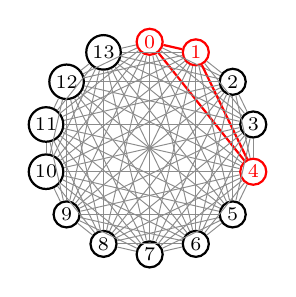
\begin{tikzpicture}[
  thick,
  baseline=(current bounding box.north),
  vertex/.style={circle,draw,inner sep=1.2pt,font=\scriptsize},
  svertex/.style={circle,draw=red,text=red,inner sep=1.2pt,font=\scriptsize}
]
  \node[svertex] (v0) at (0.000,1.350) {0};
  \node[svertex] (v1) at (0.586,1.216) {1};
  \node[vertex] (v2) at (1.055,0.842) {2};
  \node[vertex] (v3) at (1.316,0.300) {3};
  \node[svertex] (v4) at (1.316,-0.300) {4};
  \node[vertex] (v5) at (1.055,-0.842) {5};
  \node[vertex] (v6) at (0.586,-1.216) {6};
  \node[vertex] (v7) at (0.000,-1.350) {7};
  \node[vertex] (v8) at (-0.586,-1.216) {8};
  \node[vertex] (v9) at (-1.055,-0.842) {9};
  \node[vertex] (v10) at (-1.316,-0.300) {10};
  \node[vertex] (v11) at (-1.316,0.300) {11};
  \node[vertex] (v12) at (-1.055,0.842) {12};
  \node[vertex] (v13) at (-0.586,1.216) {13};
  \draw[red] (v0) -- (v1);
  \draw[black!45,line width=0.35pt] (v0) -- (v2);
  \draw[black!45,line width=0.35pt] (v0) -- (v3);
  \draw[red] (v0) -- (v4);
  \draw[black!45,line width=0.35pt] (v0) -- (v5);
  \draw[black!45,line width=0.35pt] (v0) -- (v6);
  \draw[black!45,line width=0.35pt] (v0) -- (v7);
  \draw[black!45,line width=0.35pt] (v0) -- (v8);
  \draw[black!45,line width=0.35pt] (v0) -- (v9);
  \draw[black!45,line width=0.35pt] (v0) -- (v10);
  \draw[black!45,line width=0.35pt] (v0) -- (v11);
  \draw[black!45,line width=0.35pt] (v0) -- (v12);
  \draw[black!45,line width=0.35pt] (v0) -- (v13);
  \draw[black!45,line width=0.35pt] (v1) -- (v2);
  \draw[black!45,line width=0.35pt] (v1) -- (v3);
  \draw[red] (v1) -- (v4);
  \draw[black!45,line width=0.35pt] (v1) -- (v5);
  \draw[black!45,line width=0.35pt] (v1) -- (v6);
  \draw[black!45,line width=0.35pt] (v1) -- (v7);
  \draw[black!45,line width=0.35pt] (v1) -- (v8);
  \draw[black!45,line width=0.35pt] (v1) -- (v9);
  \draw[black!45,line width=0.35pt] (v1) -- (v10);
  \draw[black!45,line width=0.35pt] (v1) -- (v11);
  \draw[black!45,line width=0.35pt] (v1) -- (v12);
  \draw[black!45,line width=0.35pt] (v1) -- (v13);
  \draw[black!45,line width=0.35pt] (v2) -- (v3);
  \draw[black!45,line width=0.35pt] (v2) -- (v4);
  \draw[black!45,line width=0.35pt] (v2) -- (v5);
  \draw[black!45,line width=0.35pt] (v2) -- (v6);
  \draw[black!45,line width=0.35pt] (v2) -- (v7);
  \draw[black!45,line width=0.35pt] (v2) -- (v8);
  \draw[black!45,line width=0.35pt] (v2) -- (v9);
  \draw[black!45,line width=0.35pt] (v2) -- (v10);
  \draw[black!45,line width=0.35pt] (v2) -- (v11);
  \draw[black!45,line width=0.35pt] (v2) -- (v12);
  \draw[black!45,line width=0.35pt] (v2) -- (v13);
  \draw[black!45,line width=0.35pt] (v3) -- (v4);
  \draw[black!45,line width=0.35pt] (v3) -- (v5);
  \draw[black!45,line width=0.35pt] (v3) -- (v6);
  \draw[black!45,line width=0.35pt] (v3) -- (v7);
  \draw[black!45,line width=0.35pt] (v3) -- (v8);
  \draw[black!45,line width=0.35pt] (v3) -- (v9);
  \draw[black!45,line width=0.35pt] (v3) -- (v10);
  \draw[black!45,line width=0.35pt] (v3) -- (v11);
  \draw[black!45,line width=0.35pt] (v3) -- (v12);
  \draw[black!45,line width=0.35pt] (v3) -- (v13);
  \draw[black!45,line width=0.35pt] (v4) -- (v5);
  \draw[black!45,line width=0.35pt] (v4) -- (v6);
  \draw[black!45,line width=0.35pt] (v4) -- (v7);
  \draw[black!45,line width=0.35pt] (v4) -- (v8);
  \draw[black!45,line width=0.35pt] (v4) -- (v9);
  \draw[black!45,line width=0.35pt] (v4) -- (v10);
  \draw[black!45,line width=0.35pt] (v4) -- (v11);
  \draw[black!45,line width=0.35pt] (v4) -- (v12);
  \draw[black!45,line width=0.35pt] (v4) -- (v13);
  \draw[black!45,line width=0.35pt] (v5) -- (v6);
  \draw[black!45,line width=0.35pt] (v5) -- (v7);
  \draw[black!45,line width=0.35pt] (v5) -- (v8);
  \draw[black!45,line width=0.35pt] (v5) -- (v9);
  \draw[black!45,line width=0.35pt] (v5) -- (v10);
  \draw[black!45,line width=0.35pt] (v5) -- (v11);
  \draw[black!45,line width=0.35pt] (v5) -- (v12);
  \draw[black!45,line width=0.35pt] (v5) -- (v13);
  \draw[black!45,line width=0.35pt] (v6) -- (v7);
  \draw[black!45,line width=0.35pt] (v6) -- (v8);
  \draw[black!45,line width=0.35pt] (v6) -- (v9);
  \draw[black!45,line width=0.35pt] (v6) -- (v10);
  \draw[black!45,line width=0.35pt] (v6) -- (v11);
  \draw[black!45,line width=0.35pt] (v6) -- (v12);
  \draw[black!45,line width=0.35pt] (v6) -- (v13);
  \draw[black!45,line width=0.35pt] (v7) -- (v8);
  \draw[black!45,line width=0.35pt] (v7) -- (v9);
  \draw[black!45,line width=0.35pt] (v7) -- (v10);
  \draw[black!45,line width=0.35pt] (v7) -- (v11);
  \draw[black!45,line width=0.35pt] (v7) -- (v12);
  \draw[black!45,line width=0.35pt] (v7) -- (v13);
  \draw[black!45,line width=0.35pt] (v8) -- (v9);
  \draw[black!45,line width=0.35pt] (v8) -- (v10);
  \draw[black!45,line width=0.35pt] (v8) -- (v11);
  \draw[black!45,line width=0.35pt] (v8) -- (v12);
  \draw[black!45,line width=0.35pt] (v8) -- (v13);
  \draw[black!45,line width=0.35pt] (v9) -- (v10);
  \draw[black!45,line width=0.35pt] (v9) -- (v11);
  \draw[black!45,line width=0.35pt] (v9) -- (v12);
  \draw[black!45,line width=0.35pt] (v9) -- (v13);
  \draw[black!45,line width=0.35pt] (v10) -- (v11);
  \draw[black!45,line width=0.35pt] (v10) -- (v12);
  \draw[black!45,line width=0.35pt] (v10) -- (v13);
  \draw[black!45,line width=0.35pt] (v11) -- (v12);
  \draw[black!45,line width=0.35pt] (v11) -- (v13);
  \draw[black!45,line width=0.35pt] (v12) -- (v13);
\end{tikzpicture}
\end{minipage}
\par\smallskip Jumps in $E(S)$: $J=\{1,3,4\}$
\par $b_{01} + b_{14} + b_{04} \le d_m(|S|)=d_{3}(3)=2$
\par $y_{1} + y_{3} + y_{4} \le 2$
\end{center}

Each drawing below is a circulant graph $G_{L}$ for a non-empty $L\subseteq J$ with edges $E(L)=\{\{i,j\}\mid i,j\in V,\ \min((i-j)\bmod t,\,(j-i)\bmod t)\in L\}$.
For each graph, we show $|E(L)\cap E(S)|$ and put $\textcolor{green!60!black}{\checkmark}$ iff $|E(L)\cap E(S)|=d_m(|S|)$; otherwise $\textcolor{red}{\boldsymbol{\times}}$.
When a checked graph is minimal under single-jump deletion, we append $\textbf{MIN}$ right after the checkmark.
Only graphs that pass the check are shown. 
Recipe mode: shown graphs are built directly as CORE graphs (all active jumps except one), plus graphs obtained by adding free jumps ($a_j=0$) only to the first CORE graph. $Y$, $Y^{+}$, and rank are computed only from this shown set.

\noindent
\begin{minipage}[t]{0.31\textwidth}
\centering
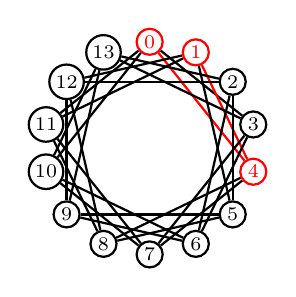
\begin{tikzpicture}[
  thick,  vertex/.style={circle,draw,inner sep=1.2pt,font=\scriptsize},  svertex/.style={circle,draw=red,text=red,inner sep=1.2pt,font=\scriptsize},  baseline=(current bounding box.north)
]
  \node[svertex] (v0) at (0.000,1.350) {0};
  \node[svertex] (v1) at (0.586,1.216) {1};
  \node[vertex] (v2) at (1.055,0.842) {2};
  \node[vertex] (v3) at (1.316,0.300) {3};
  \node[svertex] (v4) at (1.316,-0.300) {4};
  \node[vertex] (v5) at (1.055,-0.842) {5};
  \node[vertex] (v6) at (0.586,-1.216) {6};
  \node[vertex] (v7) at (0.000,-1.350) {7};
  \node[vertex] (v8) at (-0.586,-1.216) {8};
  \node[vertex] (v9) at (-1.055,-0.842) {9};
  \node[vertex] (v10) at (-1.316,-0.300) {10};
  \node[vertex] (v11) at (-1.316,0.300) {11};
  \node[vertex] (v12) at (-1.055,0.842) {12};
  \node[vertex] (v13) at (-0.586,1.216) {13};
  \draw (v0) -- (v3);
  \draw[red] (v0) -- (v4);
  \draw (v0) -- (v10);
  \draw (v0) -- (v11);
  \draw[red] (v1) -- (v4);
  \draw (v1) -- (v5);
  \draw (v1) -- (v11);
  \draw (v1) -- (v12);
  \draw (v2) -- (v5);
  \draw (v2) -- (v6);
  \draw (v2) -- (v12);
  \draw (v2) -- (v13);
  \draw (v3) -- (v6);
  \draw (v3) -- (v7);
  \draw (v3) -- (v13);
  \draw (v4) -- (v7);
  \draw (v4) -- (v8);
  \draw (v5) -- (v8);
  \draw (v5) -- (v9);
  \draw (v6) -- (v9);
  \draw (v6) -- (v10);
  \draw (v7) -- (v10);
  \draw (v7) -- (v11);
  \draw (v8) -- (v11);
  \draw (v8) -- (v12);
  \draw (v9) -- (v12);
  \draw (v9) -- (v13);
  \draw (v10) -- (v13);
\end{tikzpicture}
\par\smallskip Graph 1
\par $L=\{\textcolor{red}{3},\textcolor{red}{4}\}$
\par $y=\left(\textcolor{red}{0},0,\textcolor{red}{1},\textcolor{red}{1},0,0,0\right)$
\par $|E(L)\cap E(S)|=2\;\;\textcolor{green!60!black}{\checkmark}\;\textbf{MIN}$
\end{minipage}\hfill\begin{minipage}[t]{0.31\textwidth}
\centering
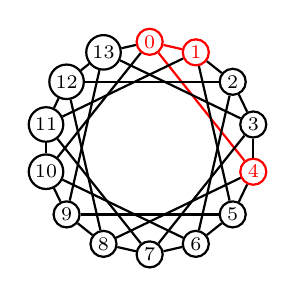
\begin{tikzpicture}[
  thick,  vertex/.style={circle,draw,inner sep=1.2pt,font=\scriptsize},  svertex/.style={circle,draw=red,text=red,inner sep=1.2pt,font=\scriptsize},  baseline=(current bounding box.north)
]
  \node[svertex] (v0) at (0.000,1.350) {0};
  \node[svertex] (v1) at (0.586,1.216) {1};
  \node[vertex] (v2) at (1.055,0.842) {2};
  \node[vertex] (v3) at (1.316,0.300) {3};
  \node[svertex] (v4) at (1.316,-0.300) {4};
  \node[vertex] (v5) at (1.055,-0.842) {5};
  \node[vertex] (v6) at (0.586,-1.216) {6};
  \node[vertex] (v7) at (0.000,-1.350) {7};
  \node[vertex] (v8) at (-0.586,-1.216) {8};
  \node[vertex] (v9) at (-1.055,-0.842) {9};
  \node[vertex] (v10) at (-1.316,-0.300) {10};
  \node[vertex] (v11) at (-1.316,0.300) {11};
  \node[vertex] (v12) at (-1.055,0.842) {12};
  \node[vertex] (v13) at (-0.586,1.216) {13};
  \draw[red] (v0) -- (v1);
  \draw[red] (v0) -- (v4);
  \draw (v0) -- (v10);
  \draw (v0) -- (v13);
  \draw (v1) -- (v2);
  \draw (v1) -- (v5);
  \draw (v1) -- (v11);
  \draw (v2) -- (v3);
  \draw (v2) -- (v6);
  \draw (v2) -- (v12);
  \draw (v3) -- (v4);
  \draw (v3) -- (v7);
  \draw (v3) -- (v13);
  \draw (v4) -- (v5);
  \draw (v4) -- (v8);
  \draw (v5) -- (v6);
  \draw (v5) -- (v9);
  \draw (v6) -- (v7);
  \draw (v6) -- (v10);
  \draw (v7) -- (v8);
  \draw (v7) -- (v11);
  \draw (v8) -- (v9);
  \draw (v8) -- (v12);
  \draw (v9) -- (v10);
  \draw (v9) -- (v13);
  \draw (v10) -- (v11);
  \draw (v11) -- (v12);
  \draw (v12) -- (v13);
\end{tikzpicture}
\par\smallskip Graph 2
\par $L=\{\textcolor{red}{1},\textcolor{red}{4}\}$
\par $y=\left(\textcolor{red}{1},0,\textcolor{red}{0},\textcolor{red}{1},0,0,0\right)$
\par $|E(L)\cap E(S)|=2\;\;\textcolor{green!60!black}{\checkmark}\;\textbf{MIN}$
\end{minipage}\hfill\begin{minipage}[t]{0.31\textwidth}
\centering
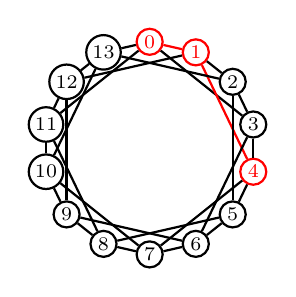
\begin{tikzpicture}[
  thick,  vertex/.style={circle,draw,inner sep=1.2pt,font=\scriptsize},  svertex/.style={circle,draw=red,text=red,inner sep=1.2pt,font=\scriptsize},  baseline=(current bounding box.north)
]
  \node[svertex] (v0) at (0.000,1.350) {0};
  \node[svertex] (v1) at (0.586,1.216) {1};
  \node[vertex] (v2) at (1.055,0.842) {2};
  \node[vertex] (v3) at (1.316,0.300) {3};
  \node[svertex] (v4) at (1.316,-0.300) {4};
  \node[vertex] (v5) at (1.055,-0.842) {5};
  \node[vertex] (v6) at (0.586,-1.216) {6};
  \node[vertex] (v7) at (0.000,-1.350) {7};
  \node[vertex] (v8) at (-0.586,-1.216) {8};
  \node[vertex] (v9) at (-1.055,-0.842) {9};
  \node[vertex] (v10) at (-1.316,-0.300) {10};
  \node[vertex] (v11) at (-1.316,0.300) {11};
  \node[vertex] (v12) at (-1.055,0.842) {12};
  \node[vertex] (v13) at (-0.586,1.216) {13};
  \draw[red] (v0) -- (v1);
  \draw (v0) -- (v3);
  \draw (v0) -- (v11);
  \draw (v0) -- (v13);
  \draw (v1) -- (v2);
  \draw[red] (v1) -- (v4);
  \draw (v1) -- (v12);
  \draw (v2) -- (v3);
  \draw (v2) -- (v5);
  \draw (v2) -- (v13);
  \draw (v3) -- (v4);
  \draw (v3) -- (v6);
  \draw (v4) -- (v5);
  \draw (v4) -- (v7);
  \draw (v5) -- (v6);
  \draw (v5) -- (v8);
  \draw (v6) -- (v7);
  \draw (v6) -- (v9);
  \draw (v7) -- (v8);
  \draw (v7) -- (v10);
  \draw (v8) -- (v9);
  \draw (v8) -- (v11);
  \draw (v9) -- (v10);
  \draw (v9) -- (v12);
  \draw (v10) -- (v11);
  \draw (v10) -- (v13);
  \draw (v11) -- (v12);
  \draw (v12) -- (v13);
\end{tikzpicture}
\par\smallskip Graph 3
\par $L=\{\textcolor{red}{1},\textcolor{red}{3}\}$
\par $y=\left(\textcolor{red}{1},0,\textcolor{red}{1},\textcolor{red}{0},0,0,0\right)$
\par $|E(L)\cap E(S)|=2\;\;\textcolor{green!60!black}{\checkmark}\;\textbf{MIN}$
\end{minipage}
\par\medskip
\noindent
\begin{minipage}[t]{0.31\textwidth}
\centering
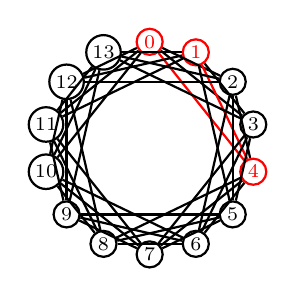
\begin{tikzpicture}[
  thick,  vertex/.style={circle,draw,inner sep=1.2pt,font=\scriptsize},  svertex/.style={circle,draw=red,text=red,inner sep=1.2pt,font=\scriptsize},  baseline=(current bounding box.north)
]
  \node[svertex] (v0) at (0.000,1.350) {0};
  \node[svertex] (v1) at (0.586,1.216) {1};
  \node[vertex] (v2) at (1.055,0.842) {2};
  \node[vertex] (v3) at (1.316,0.300) {3};
  \node[svertex] (v4) at (1.316,-0.300) {4};
  \node[vertex] (v5) at (1.055,-0.842) {5};
  \node[vertex] (v6) at (0.586,-1.216) {6};
  \node[vertex] (v7) at (0.000,-1.350) {7};
  \node[vertex] (v8) at (-0.586,-1.216) {8};
  \node[vertex] (v9) at (-1.055,-0.842) {9};
  \node[vertex] (v10) at (-1.316,-0.300) {10};
  \node[vertex] (v11) at (-1.316,0.300) {11};
  \node[vertex] (v12) at (-1.055,0.842) {12};
  \node[vertex] (v13) at (-0.586,1.216) {13};
  \draw (v0) -- (v2);
  \draw (v0) -- (v3);
  \draw[red] (v0) -- (v4);
  \draw (v0) -- (v10);
  \draw (v0) -- (v11);
  \draw (v0) -- (v12);
  \draw (v1) -- (v3);
  \draw[red] (v1) -- (v4);
  \draw (v1) -- (v5);
  \draw (v1) -- (v11);
  \draw (v1) -- (v12);
  \draw (v1) -- (v13);
  \draw (v2) -- (v4);
  \draw (v2) -- (v5);
  \draw (v2) -- (v6);
  \draw (v2) -- (v12);
  \draw (v2) -- (v13);
  \draw (v3) -- (v5);
  \draw (v3) -- (v6);
  \draw (v3) -- (v7);
  \draw (v3) -- (v13);
  \draw (v4) -- (v6);
  \draw (v4) -- (v7);
  \draw (v4) -- (v8);
  \draw (v5) -- (v7);
  \draw (v5) -- (v8);
  \draw (v5) -- (v9);
  \draw (v6) -- (v8);
  \draw (v6) -- (v9);
  \draw (v6) -- (v10);
  \draw (v7) -- (v9);
  \draw (v7) -- (v10);
  \draw (v7) -- (v11);
  \draw (v8) -- (v10);
  \draw (v8) -- (v11);
  \draw (v8) -- (v12);
  \draw (v9) -- (v11);
  \draw (v9) -- (v12);
  \draw (v9) -- (v13);
  \draw (v10) -- (v12);
  \draw (v10) -- (v13);
  \draw (v11) -- (v13);
\end{tikzpicture}
\par\smallskip Graph 4
\par $L=\{2,\textcolor{red}{3},\textcolor{red}{4}\}$
\par $y=\left(\textcolor{red}{0},1,\textcolor{red}{1},\textcolor{red}{1},0,0,0\right)$
\par $|E(L)\cap E(S)|=2\;\;\textcolor{green!60!black}{\checkmark}$
\end{minipage}\hfill\begin{minipage}[t]{0.31\textwidth}
\centering
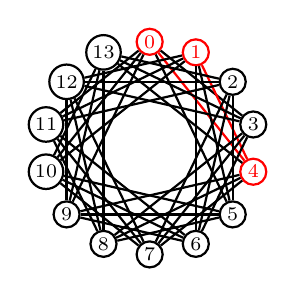
\begin{tikzpicture}[
  thick,  vertex/.style={circle,draw,inner sep=1.2pt,font=\scriptsize},  svertex/.style={circle,draw=red,text=red,inner sep=1.2pt,font=\scriptsize},  baseline=(current bounding box.north)
]
  \node[svertex] (v0) at (0.000,1.350) {0};
  \node[svertex] (v1) at (0.586,1.216) {1};
  \node[vertex] (v2) at (1.055,0.842) {2};
  \node[vertex] (v3) at (1.316,0.300) {3};
  \node[svertex] (v4) at (1.316,-0.300) {4};
  \node[vertex] (v5) at (1.055,-0.842) {5};
  \node[vertex] (v6) at (0.586,-1.216) {6};
  \node[vertex] (v7) at (0.000,-1.350) {7};
  \node[vertex] (v8) at (-0.586,-1.216) {8};
  \node[vertex] (v9) at (-1.055,-0.842) {9};
  \node[vertex] (v10) at (-1.316,-0.300) {10};
  \node[vertex] (v11) at (-1.316,0.300) {11};
  \node[vertex] (v12) at (-1.055,0.842) {12};
  \node[vertex] (v13) at (-0.586,1.216) {13};
  \draw (v0) -- (v3);
  \draw[red] (v0) -- (v4);
  \draw (v0) -- (v5);
  \draw (v0) -- (v9);
  \draw (v0) -- (v10);
  \draw (v0) -- (v11);
  \draw[red] (v1) -- (v4);
  \draw (v1) -- (v5);
  \draw (v1) -- (v6);
  \draw (v1) -- (v10);
  \draw (v1) -- (v11);
  \draw (v1) -- (v12);
  \draw (v2) -- (v5);
  \draw (v2) -- (v6);
  \draw (v2) -- (v7);
  \draw (v2) -- (v11);
  \draw (v2) -- (v12);
  \draw (v2) -- (v13);
  \draw (v3) -- (v6);
  \draw (v3) -- (v7);
  \draw (v3) -- (v8);
  \draw (v3) -- (v12);
  \draw (v3) -- (v13);
  \draw (v4) -- (v7);
  \draw (v4) -- (v8);
  \draw (v4) -- (v9);
  \draw (v4) -- (v13);
  \draw (v5) -- (v8);
  \draw (v5) -- (v9);
  \draw (v5) -- (v10);
  \draw (v6) -- (v9);
  \draw (v6) -- (v10);
  \draw (v6) -- (v11);
  \draw (v7) -- (v10);
  \draw (v7) -- (v11);
  \draw (v7) -- (v12);
  \draw (v8) -- (v11);
  \draw (v8) -- (v12);
  \draw (v8) -- (v13);
  \draw (v9) -- (v12);
  \draw (v9) -- (v13);
  \draw (v10) -- (v13);
\end{tikzpicture}
\par\smallskip Graph 5
\par $L=\{\textcolor{red}{3},\textcolor{red}{4},5\}$
\par $y=\left(\textcolor{red}{0},0,\textcolor{red}{1},\textcolor{red}{1},1,0,0\right)$
\par $|E(L)\cap E(S)|=2\;\;\textcolor{green!60!black}{\checkmark}$
\end{minipage}\hfill\begin{minipage}[t]{0.31\textwidth}
\centering
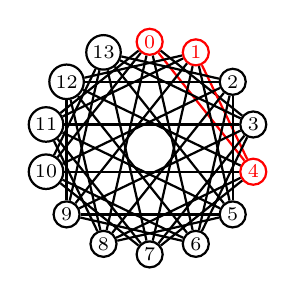
\begin{tikzpicture}[
  thick,  vertex/.style={circle,draw,inner sep=1.2pt,font=\scriptsize},  svertex/.style={circle,draw=red,text=red,inner sep=1.2pt,font=\scriptsize},  baseline=(current bounding box.north)
]
  \node[svertex] (v0) at (0.000,1.350) {0};
  \node[svertex] (v1) at (0.586,1.216) {1};
  \node[vertex] (v2) at (1.055,0.842) {2};
  \node[vertex] (v3) at (1.316,0.300) {3};
  \node[svertex] (v4) at (1.316,-0.300) {4};
  \node[vertex] (v5) at (1.055,-0.842) {5};
  \node[vertex] (v6) at (0.586,-1.216) {6};
  \node[vertex] (v7) at (0.000,-1.350) {7};
  \node[vertex] (v8) at (-0.586,-1.216) {8};
  \node[vertex] (v9) at (-1.055,-0.842) {9};
  \node[vertex] (v10) at (-1.316,-0.300) {10};
  \node[vertex] (v11) at (-1.316,0.300) {11};
  \node[vertex] (v12) at (-1.055,0.842) {12};
  \node[vertex] (v13) at (-0.586,1.216) {13};
  \draw (v0) -- (v3);
  \draw[red] (v0) -- (v4);
  \draw (v0) -- (v6);
  \draw (v0) -- (v8);
  \draw (v0) -- (v10);
  \draw (v0) -- (v11);
  \draw[red] (v1) -- (v4);
  \draw (v1) -- (v5);
  \draw (v1) -- (v7);
  \draw (v1) -- (v9);
  \draw (v1) -- (v11);
  \draw (v1) -- (v12);
  \draw (v2) -- (v5);
  \draw (v2) -- (v6);
  \draw (v2) -- (v8);
  \draw (v2) -- (v10);
  \draw (v2) -- (v12);
  \draw (v2) -- (v13);
  \draw (v3) -- (v6);
  \draw (v3) -- (v7);
  \draw (v3) -- (v9);
  \draw (v3) -- (v11);
  \draw (v3) -- (v13);
  \draw (v4) -- (v7);
  \draw (v4) -- (v8);
  \draw (v4) -- (v10);
  \draw (v4) -- (v12);
  \draw (v5) -- (v8);
  \draw (v5) -- (v9);
  \draw (v5) -- (v11);
  \draw (v5) -- (v13);
  \draw (v6) -- (v9);
  \draw (v6) -- (v10);
  \draw (v6) -- (v12);
  \draw (v7) -- (v10);
  \draw (v7) -- (v11);
  \draw (v7) -- (v13);
  \draw (v8) -- (v11);
  \draw (v8) -- (v12);
  \draw (v9) -- (v12);
  \draw (v9) -- (v13);
  \draw (v10) -- (v13);
\end{tikzpicture}
\par\smallskip Graph 6
\par $L=\{\textcolor{red}{3},\textcolor{red}{4},6\}$
\par $y=\left(\textcolor{red}{0},0,\textcolor{red}{1},\textcolor{red}{1},0,1,0\right)$
\par $|E(L)\cap E(S)|=2\;\;\textcolor{green!60!black}{\checkmark}$
\end{minipage}
\par\medskip
\noindent
\begin{minipage}[t]{0.31\textwidth}
\centering
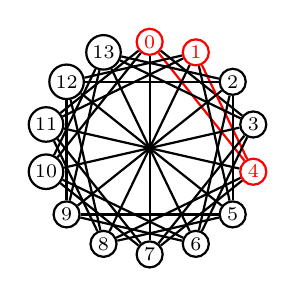
\begin{tikzpicture}[
  thick,  vertex/.style={circle,draw,inner sep=1.2pt,font=\scriptsize},  svertex/.style={circle,draw=red,text=red,inner sep=1.2pt,font=\scriptsize},  baseline=(current bounding box.north)
]
  \node[svertex] (v0) at (0.000,1.350) {0};
  \node[svertex] (v1) at (0.586,1.216) {1};
  \node[vertex] (v2) at (1.055,0.842) {2};
  \node[vertex] (v3) at (1.316,0.300) {3};
  \node[svertex] (v4) at (1.316,-0.300) {4};
  \node[vertex] (v5) at (1.055,-0.842) {5};
  \node[vertex] (v6) at (0.586,-1.216) {6};
  \node[vertex] (v7) at (0.000,-1.350) {7};
  \node[vertex] (v8) at (-0.586,-1.216) {8};
  \node[vertex] (v9) at (-1.055,-0.842) {9};
  \node[vertex] (v10) at (-1.316,-0.300) {10};
  \node[vertex] (v11) at (-1.316,0.300) {11};
  \node[vertex] (v12) at (-1.055,0.842) {12};
  \node[vertex] (v13) at (-0.586,1.216) {13};
  \draw (v0) -- (v3);
  \draw[red] (v0) -- (v4);
  \draw (v0) -- (v7);
  \draw (v0) -- (v10);
  \draw (v0) -- (v11);
  \draw[red] (v1) -- (v4);
  \draw (v1) -- (v5);
  \draw (v1) -- (v8);
  \draw (v1) -- (v11);
  \draw (v1) -- (v12);
  \draw (v2) -- (v5);
  \draw (v2) -- (v6);
  \draw (v2) -- (v9);
  \draw (v2) -- (v12);
  \draw (v2) -- (v13);
  \draw (v3) -- (v6);
  \draw (v3) -- (v7);
  \draw (v3) -- (v10);
  \draw (v3) -- (v13);
  \draw (v4) -- (v7);
  \draw (v4) -- (v8);
  \draw (v4) -- (v11);
  \draw (v5) -- (v8);
  \draw (v5) -- (v9);
  \draw (v5) -- (v12);
  \draw (v6) -- (v9);
  \draw (v6) -- (v10);
  \draw (v6) -- (v13);
  \draw (v7) -- (v10);
  \draw (v7) -- (v11);
  \draw (v8) -- (v11);
  \draw (v8) -- (v12);
  \draw (v9) -- (v12);
  \draw (v9) -- (v13);
  \draw (v10) -- (v13);
\end{tikzpicture}
\par\smallskip Graph 7
\par $L=\{\textcolor{red}{3},\textcolor{red}{4},7\}$
\par $y=\left(\textcolor{red}{0},0,\textcolor{red}{1},\textcolor{red}{1},0,0,1\right)$
\par $|E(L)\cap E(S)|=2\;\;\textcolor{green!60!black}{\checkmark}$
\end{minipage}
\par\medskip

\noindent\textbf{Matrix Data}
\par $N=7$
\par $I=\{1,2,3,4,5,6,7\}$\quad$Y=\begin{bmatrix}0 & 1 & 1 & 0 & 0 & 0 & 0 \\ 0 & 0 & 0 & 1 & 0 & 0 & 0 \\ 1 & 0 & 1 & 1 & 1 & 1 & 1 \\ 1 & 1 & 0 & 1 & 1 & 1 & 1 \\ 0 & 0 & 0 & 0 & 1 & 0 & 0 \\ 0 & 0 & 0 & 0 & 0 & 1 & 0 \\ 0 & 0 & 0 & 0 & 0 & 0 & 1\end{bmatrix}$
\par $Y^{+}=\begin{bmatrix}0 & 1 & 1 & 0 & 0 & 0 & 0 \\ 0 & 0 & 0 & 1 & 0 & 0 & 0 \\ 1 & 0 & 1 & 1 & 1 & 1 & 1 \\ 1 & 1 & 0 & 1 & 1 & 1 & 1 \\ 0 & 0 & 0 & 0 & 1 & 0 & 0 \\ 0 & 0 & 0 & 0 & 0 & 1 & 0 \\ 0 & 0 & 0 & 0 & 0 & 0 & 1 \\ 1 & 1 & 1 & 1 & 1 & 1 & 1\end{bmatrix}$\quad$\operatorname{rank}(Y^{+})=7$
\end{document}
